\newpage
\section*{RESULTADOS}
\addcontentsline{toc}{section}{RESULTADOS}
\par\refstepcounter{section}
\subsection{Pruebas en potenciales de proteínas}
\subsubsection{Clasificación de estructuras en nativas o no nativas}
\par
Los resultados de todos los potenciales en esta prueba se ven en la figura~\ref{fig:ferrada2009} donde los nuevos potenciales BSASA, SASA y BSASA+SASA no logran superar en performance a los antiguos dependientes de distancia.
En la tabla~\ref{table:f2009res} podemos ver la comparación del desempeño de todos los potenciales utilizando el método STaR (\cite{Vergara2008}), donde los potenciales BSASA,SASA y combinación BSASA+SASA tienen desempeños estadísticamente equivalentes entre si, y distintos a los potenciales de distancia, combinación distancia más conteo, y conteo.

\begin{table}[!htp]
\begin{tabular}{p{70pt} p{70pt} p{40pt} p{70pt} p{30pt} p{40pt} p{30pt}}
\hline \\
           & DD+CONTEO & BSASA         & BSASA+SASA & DD       & CONTEO   & SASA \\
DD+CONTEO  & -         & -             & -          & -        & -        & -    \\
BSASA      & \textbf{$<$0.001}  & -             & -          & -        & -        & -    \\
BSASA+SASA & \textbf{$<$0.001}  & 0.453         & -          & -        & -        & -    \\
DD         & \textbf{$<$0.001}  & \textbf{$<$0.001}      & \textbf{$<$0.001}   & -        & -        & -    \\
CONTEO     & \textbf{$<$0.001}  & \textbf{0.001}         & \textbf{$<$0.001}   & \textbf{$<$0.001} & -        & -    \\
SASA       & \textbf{$<$0.001}  & 0.284         & \textbf{$<$0.001}   & \textbf{$<$0.001} & \textbf{$<$0.001} & -    \\
\hline
\end{tabular}
\caption[Comparación entre curvas ROC para detección de estructuras nativas y no nativas]{Comparación de las curvas ROC para el desempeño de la clasificación de modelos en nativos y no nativos. Valores corresponden al p-value de la prueba no parametrica utilizada por STaR. Un p-value menor a 0.05 indica que el par no es equivalente.}
\label{table:f2009res}
\end{table}

\begin{figure}[tp]
\centering  
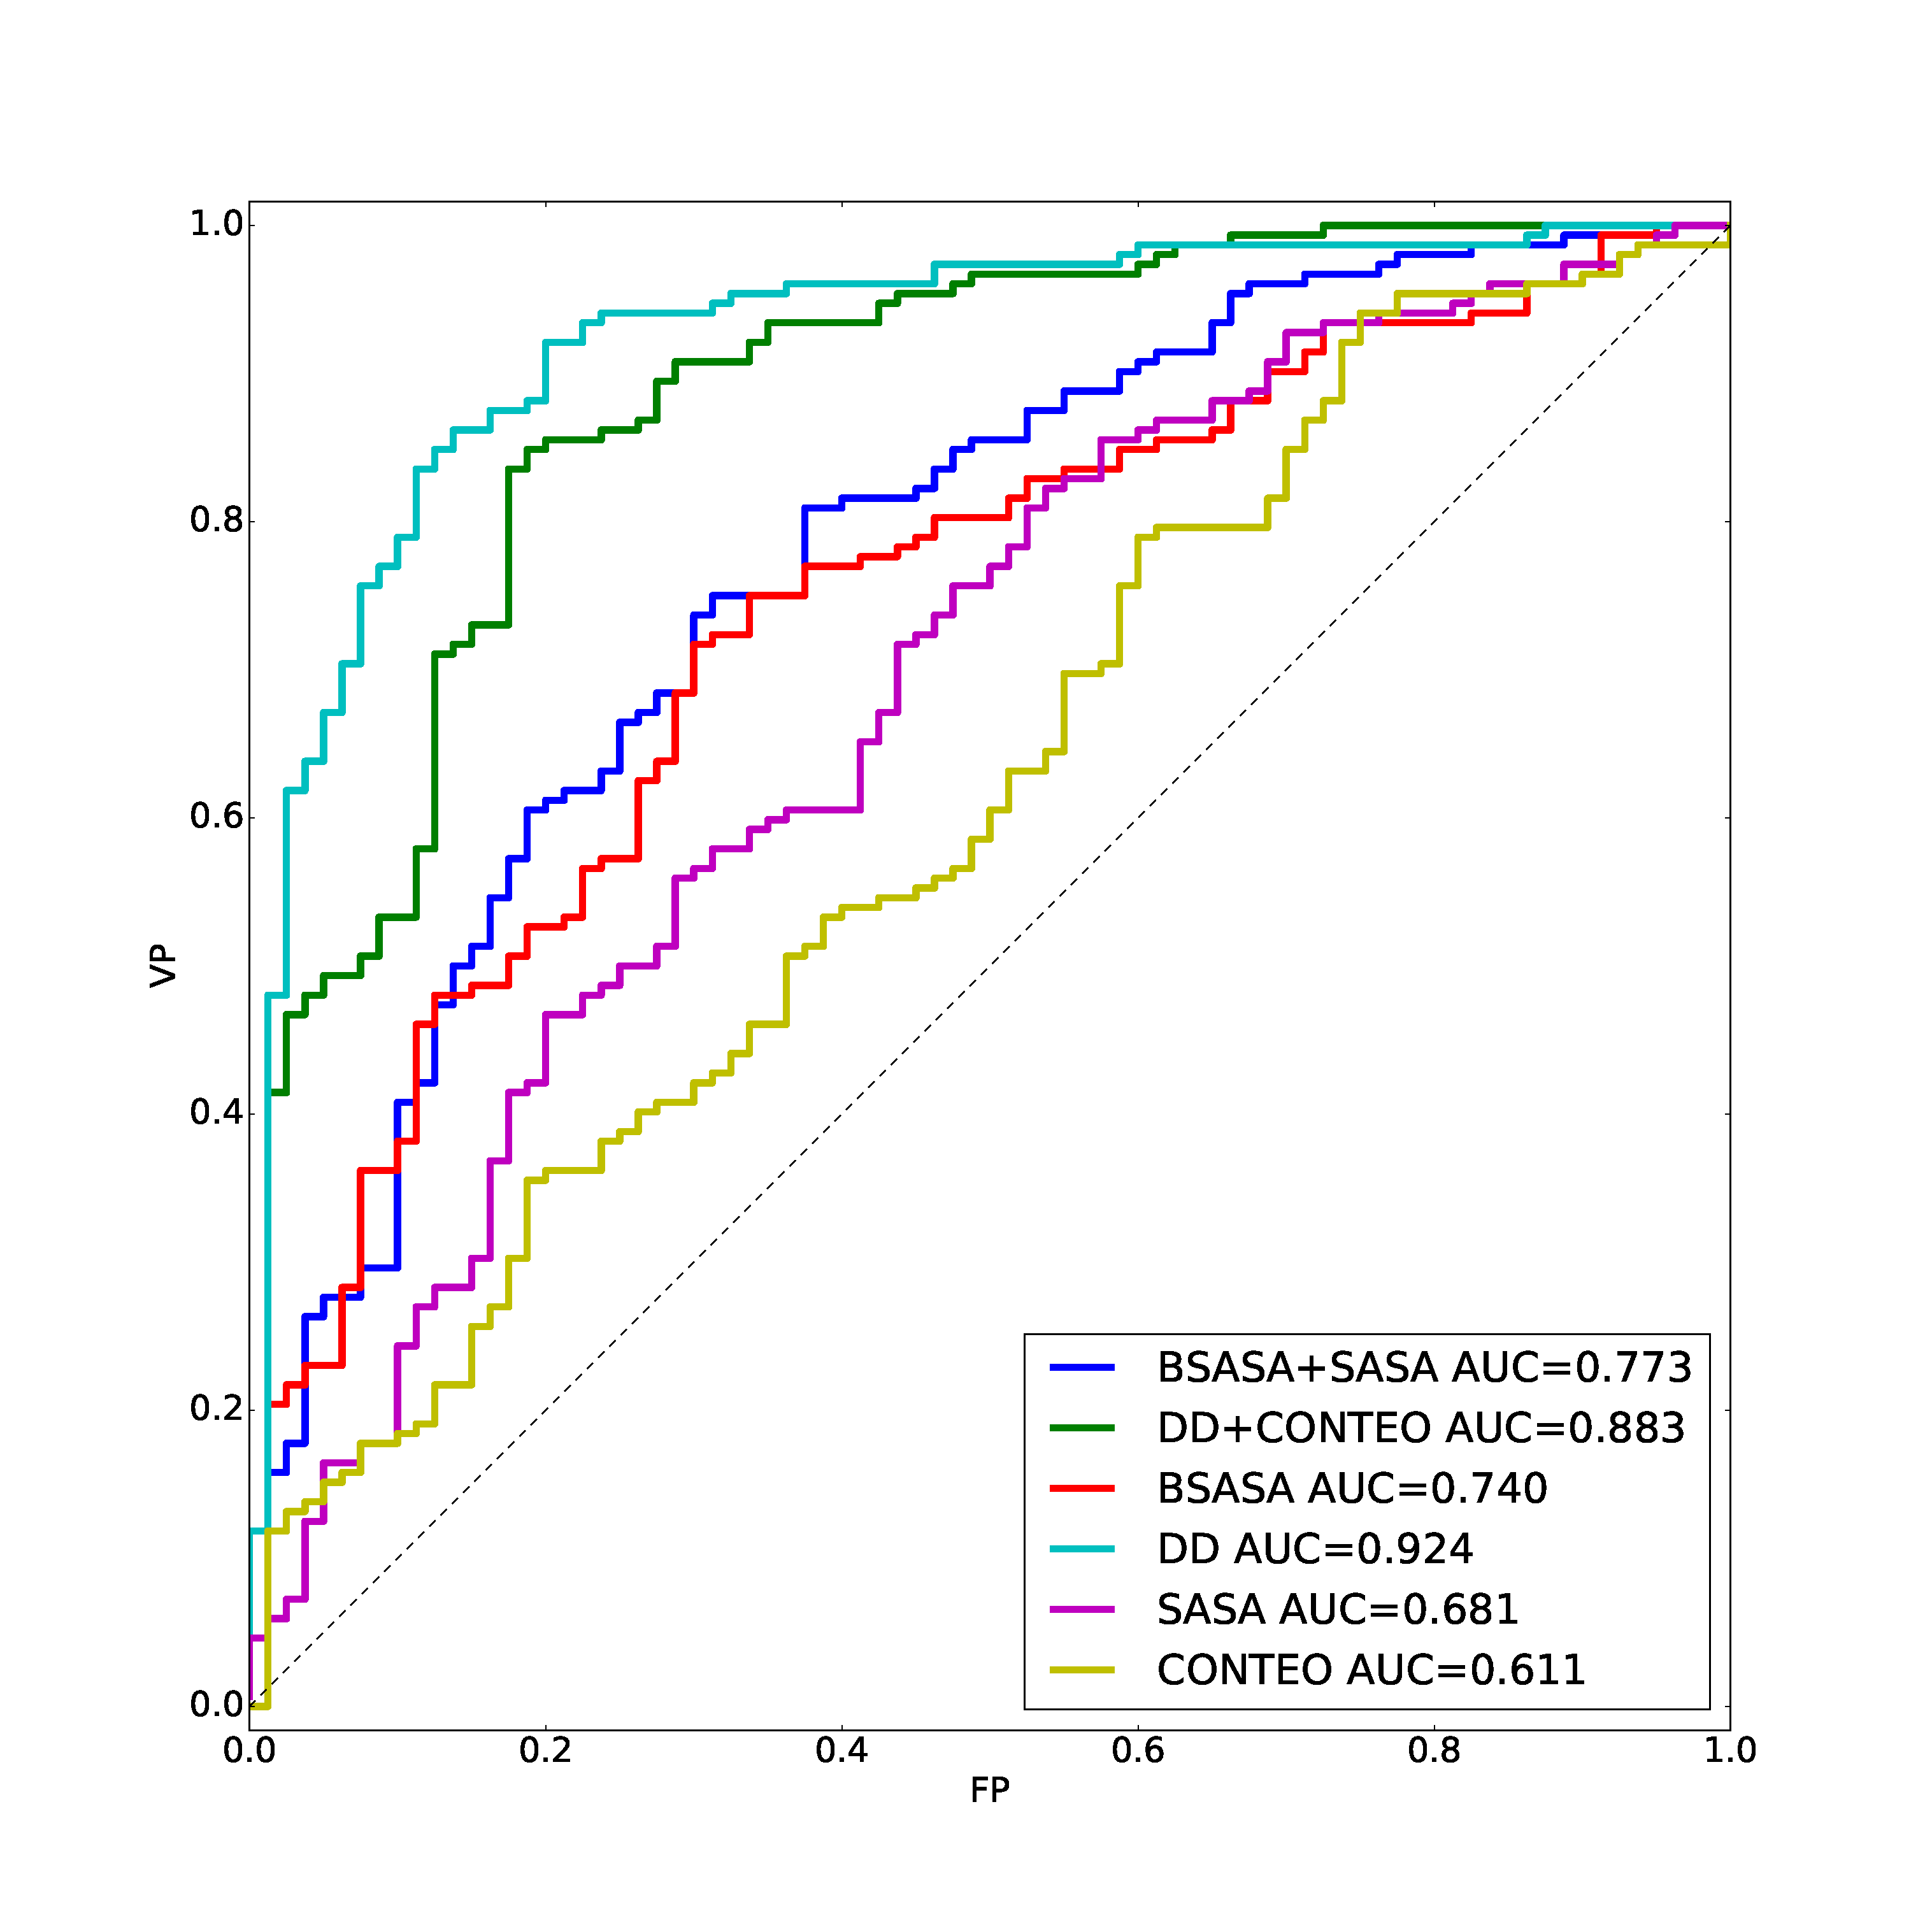
\includegraphics[width=\linewidth]{figures/resultados/prot/fold_assesment.eps}
\caption[Curvas ROC para la clasificación de estructuras en nativas y no nativas]{Curvas ROC para el desempeño de la clasificación de modelos en nativos y no nativos.}
\label{fig:ferrada2009}
\end{figure}

\subsubsection{Detección de resíduos erroneamente modelados}
\par
En la figura~\ref{fig:ferrada2007} podemos observar como los nuevos potenciales tienen mejores AUC que sus pares basados en distancias y conteos de átomos tanto como en los modelos clasificados en clase A tanto como en clase B.
Al comparar las curvas de la clase A con el método STaR en la tabla~\ref{table:f2007res} (\cite{Vergara2008}), solo hay diferencias significativas entre los potenciales de conteo y superficie SASA, considerando a los otros potenciales como equivalentes.
Mientras tanto, en los modelos clase B, en los cuáles hay más dificultad en encontrar errores, todos los potenciales se consideran distintos excepto los pares DD+CONTEO/CONTEO y BSASA/SASA.

\begin{table}[!htp]
\begin{tabular}{p{70pt} p{70pt} p{40pt} p{70pt} p{30pt} p{40pt} p{30pt}}
\hline \\
\textbf{Clase A}& DD+CONTEO  & BSASA         & BSASA+SASA & DD    & CONTEO   & SASA \\
DD+CONTEO       & -          & -             & -          & -     & -        & -    \\
BSASA           & \textbf{0.036}      & -             & -          & -     & -        & -    \\
BSASA+SASA      & 0.299      & \textbf{$<$0.001}      & -          & -     & -        & -    \\
DD              & \textbf{$<$0.001}   & 0.726         & \textbf{0.007}      & -     & -        & -    \\
CONTEO          & \textbf{0.041}      & 0.876         & \textbf{$<$0.001}   & 0.679 & -        & -    \\
SASA            & 0.801      & \textbf{0.004}         & 0.054      & 0.079 & \textbf{$<$0.001} & -    \\
\hline
\end{tabular}
\begin{tabular}{p{70pt} p{70pt} p{40pt} p{70pt} p{30pt} p{40pt} p{30pt}}
\hline \\
\textbf{Clase B}& DD+CONTEO & BSASA    & BSASA+SASA & DD       & CONTEO   & SASA \\
DD+CONTEO       & -         & -        & -          & -        & -        & -    \\
BSASA           & \textbf{$<$0.001}  & -        & -          & -        & -        & -    \\
BSASA+SASA      & \textbf{$<$0.001}  & \textbf{$<$0.001} & -          & -        & -        & -    \\
DD              & \textbf{$<$0.001}  & \textbf{$<$0.001} & \textbf{$<$0.001}   & -        & -        & -    \\
CONTEO          & 0.051     & \textbf{$<$0.001} & \textbf{$<$0.001}   & \textbf{$<$0.001} & -        & -    \\
SASA            & \textbf{$<$0.001}  & 0.732    & \textbf{$<$0.001}   & \textbf{$<$0.001} & \textbf{$<$0.001} & -    \\
\hline
\end{tabular}
\caption[Comparación entre curvas ROC de los potenciales para proteínas en detección de residuos mal modelados clase A y B]{Comparación entre curvas ROC para modelos clase A y B. Valores corresponden al p-value de la prueba no paramétrica utilizada por STaR. Un p-value menor a 0.05 indica que el par no es equivalente.}
\label{table:f2007res}
\end{table}

\begin{sidewaysfigure}[tp]
  \centering  
  \begin{subfigure}{.5\linewidth}
    \centering
    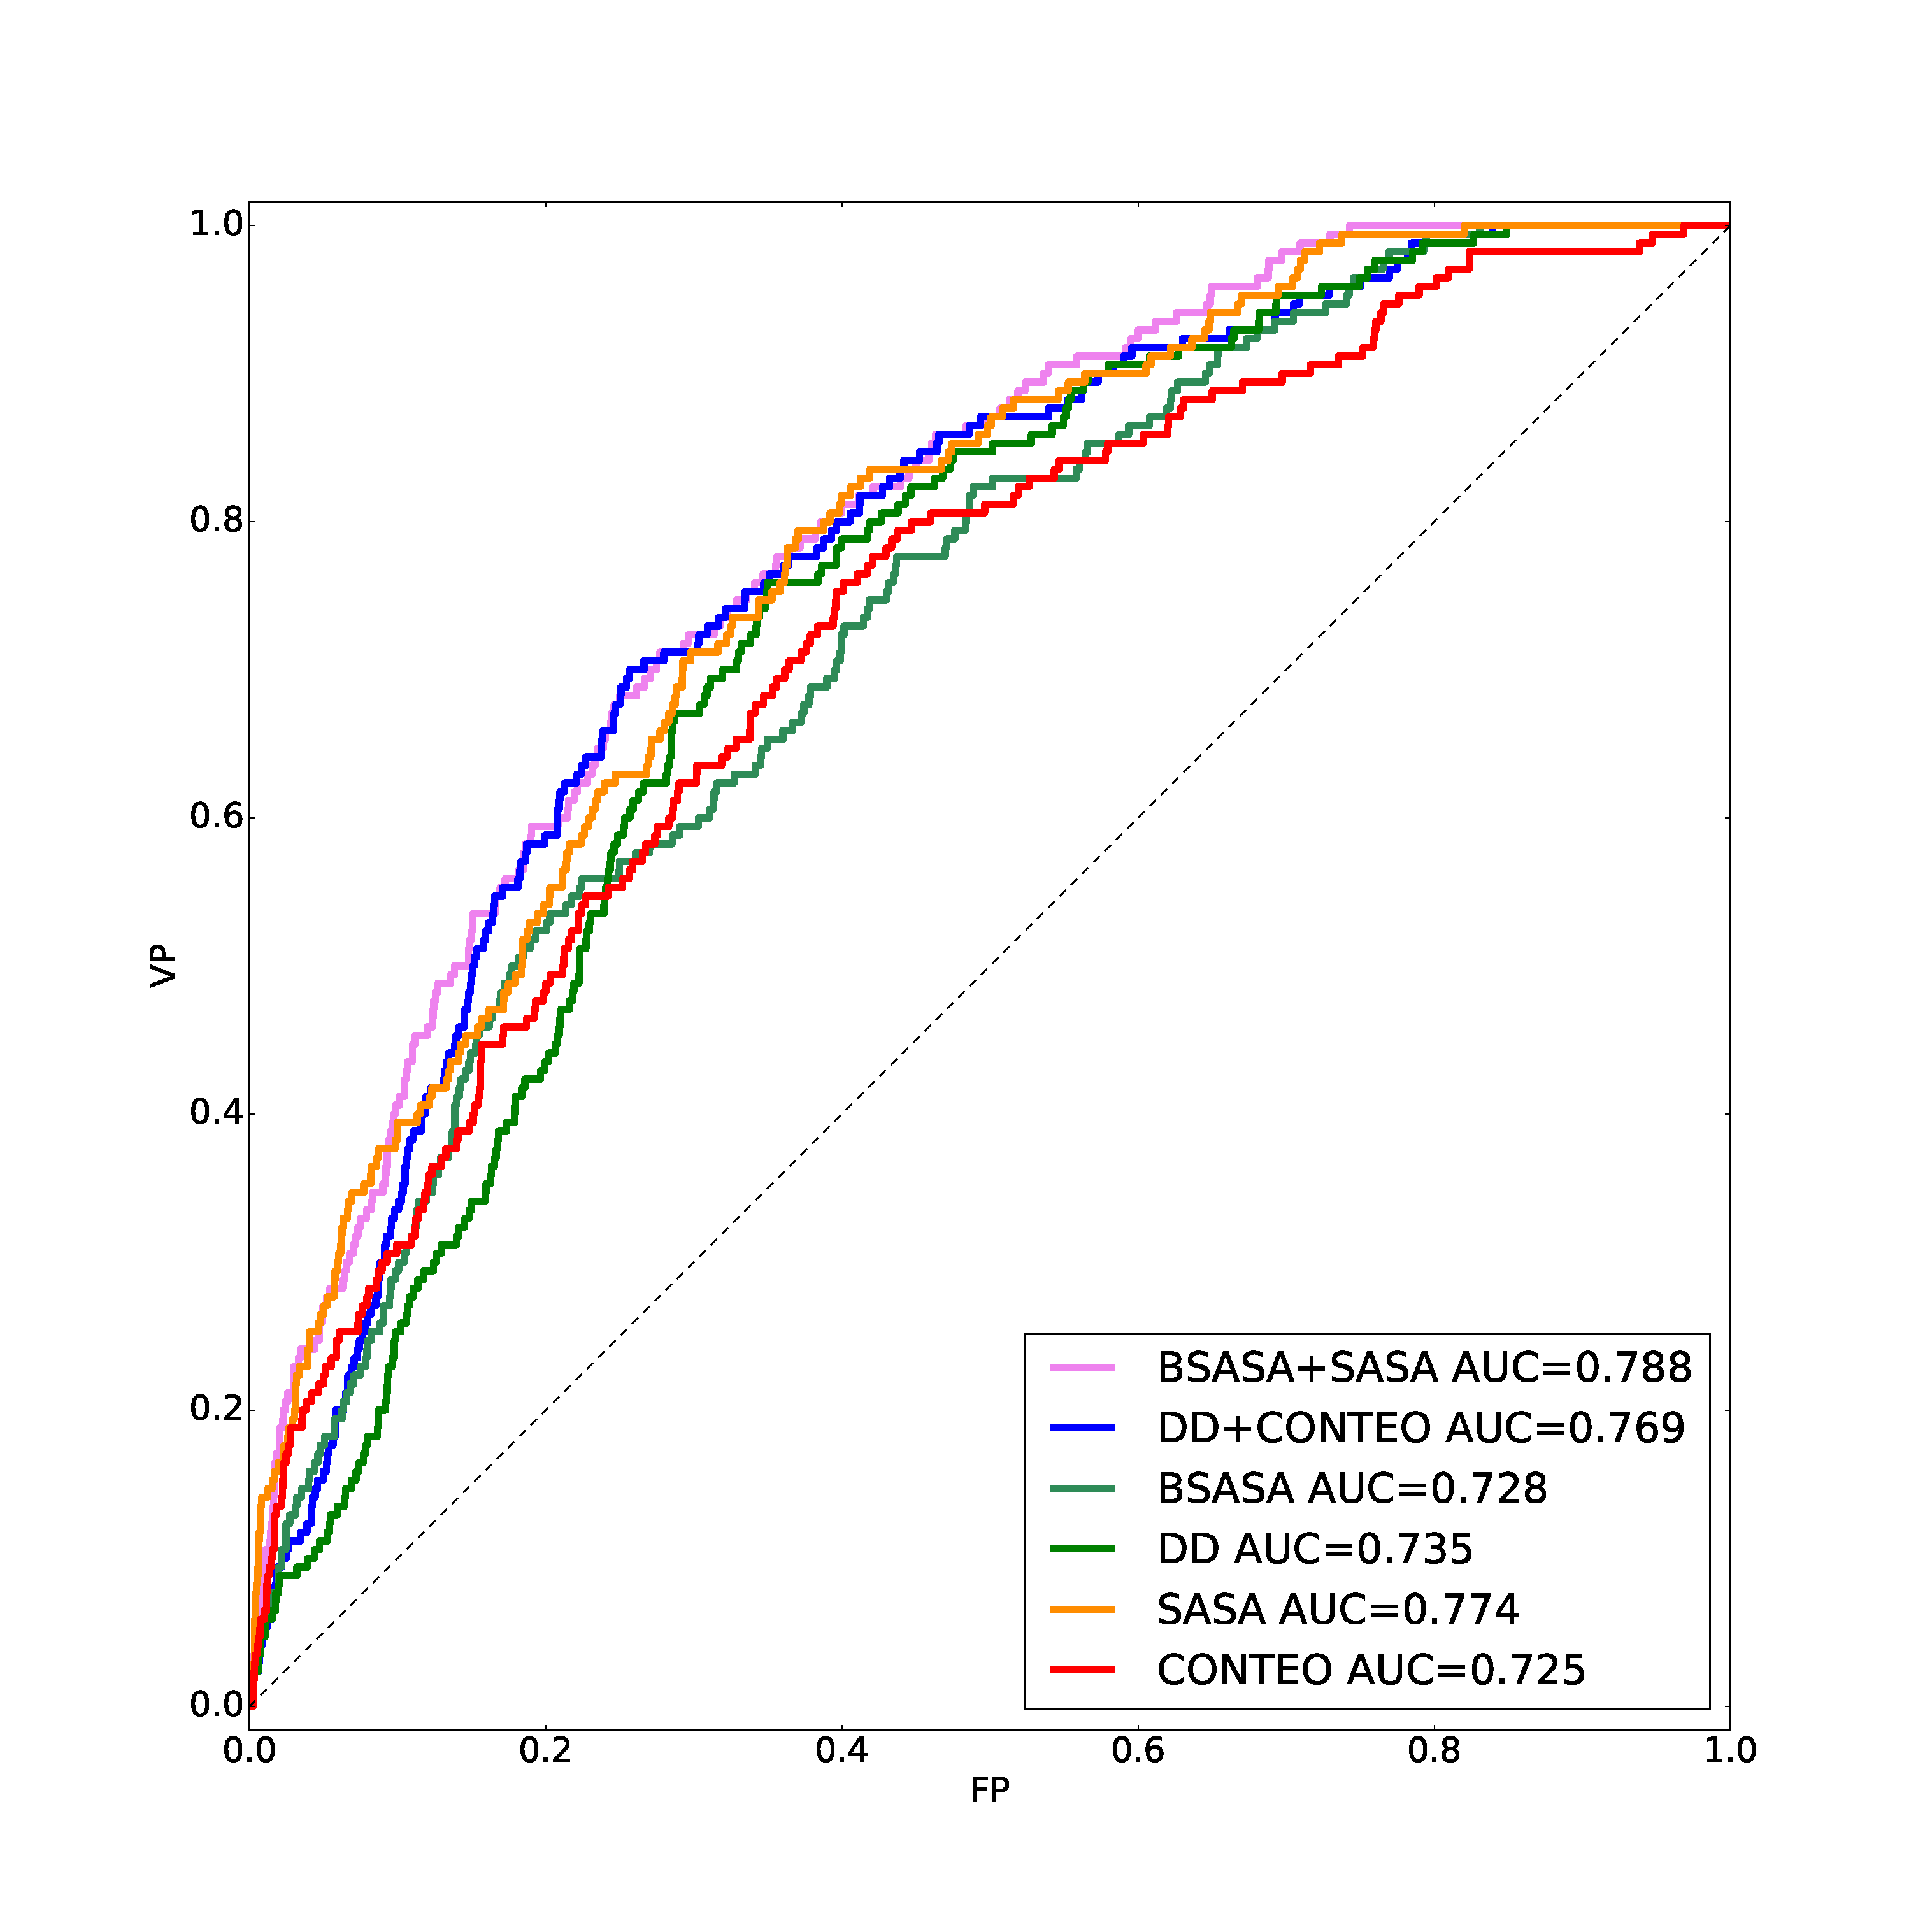
\includegraphics[width=\linewidth]{figures/resultados/prot/classA.eps}
    \caption{}
  \end{subfigure}%
~
  \begin{subfigure}{.5\linewidth}
    \centering
    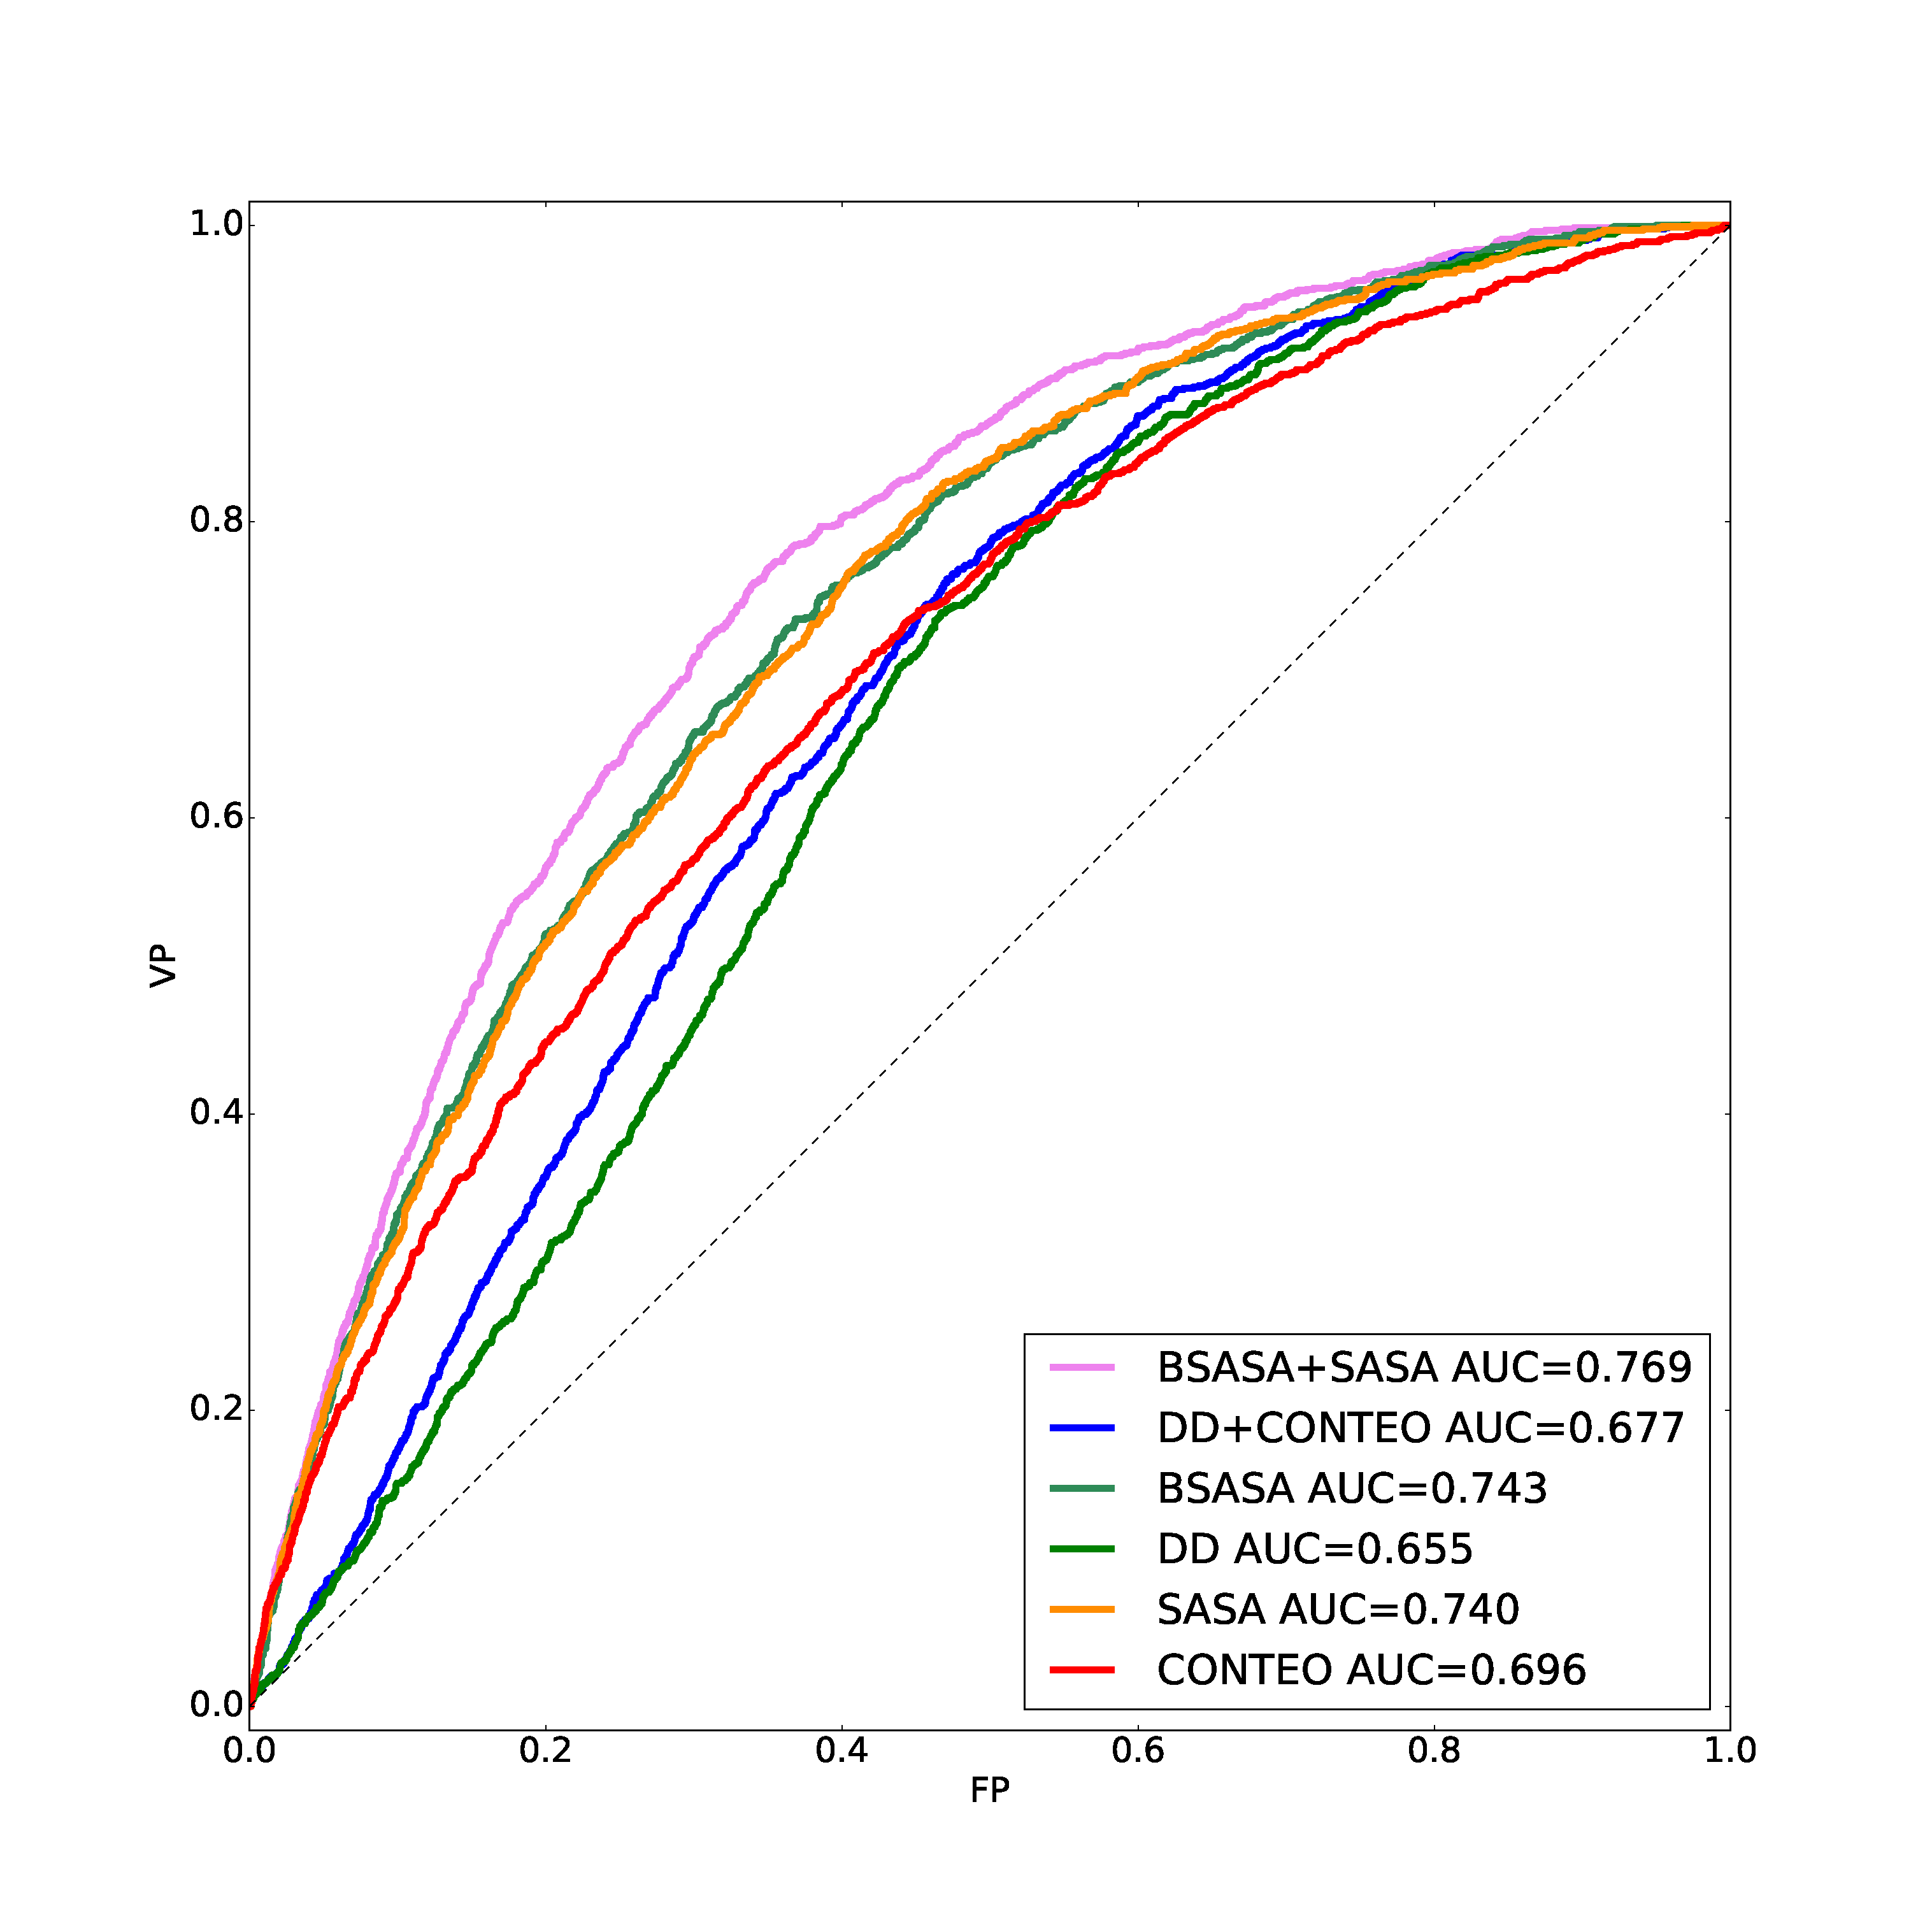
\includegraphics[width=\linewidth]{figures/resultados/prot/classB.eps}
    \caption{}
  \end{subfigure}
 
\caption[Curvas ROC para la detección de resíduos mal modelados en proteínas]{Curvas ROC para el desempeño en la detección de residuos mal modelados. En (a) se tiene la curva para las estructuras de Clase A, descritas anteriormente en métodos, mientras que en la figura (b) se tienen los resultados para las estructuras de clase B.}
\label{fig:ferrada2007}
\end{sidewaysfigure}

\cleardoublepage
\subsection{Pruebas en potenciales para ARN}
\subsubsection{Correlación entre energía y desviación estructural}
\par
En estas pruebas los nuevos potenciales tienen características de desempeño menores que los potenciales de referencia y sus combinaciones, que son RASP, CONTEO y RASP+CONTEO, como se puede observar en la figura~\ref{fig:cap2011}.
En la tabla~\ref{table:cap2011res} se tiene el p-value de las comparaciones entre todos los pares de boxplots vistos en la figura~\ref{fig:cap2011}, para RMSD tanto para GDT utilizando el test de Wilcoxon, una prueba no paramétrica alternativa al t-test de Student para datos pareados. (\cite{Wilcoxon1945})

\begin{figure}[tp]
  \centering  
  \begin{subfigure}{.8\linewidth}
    \centering
    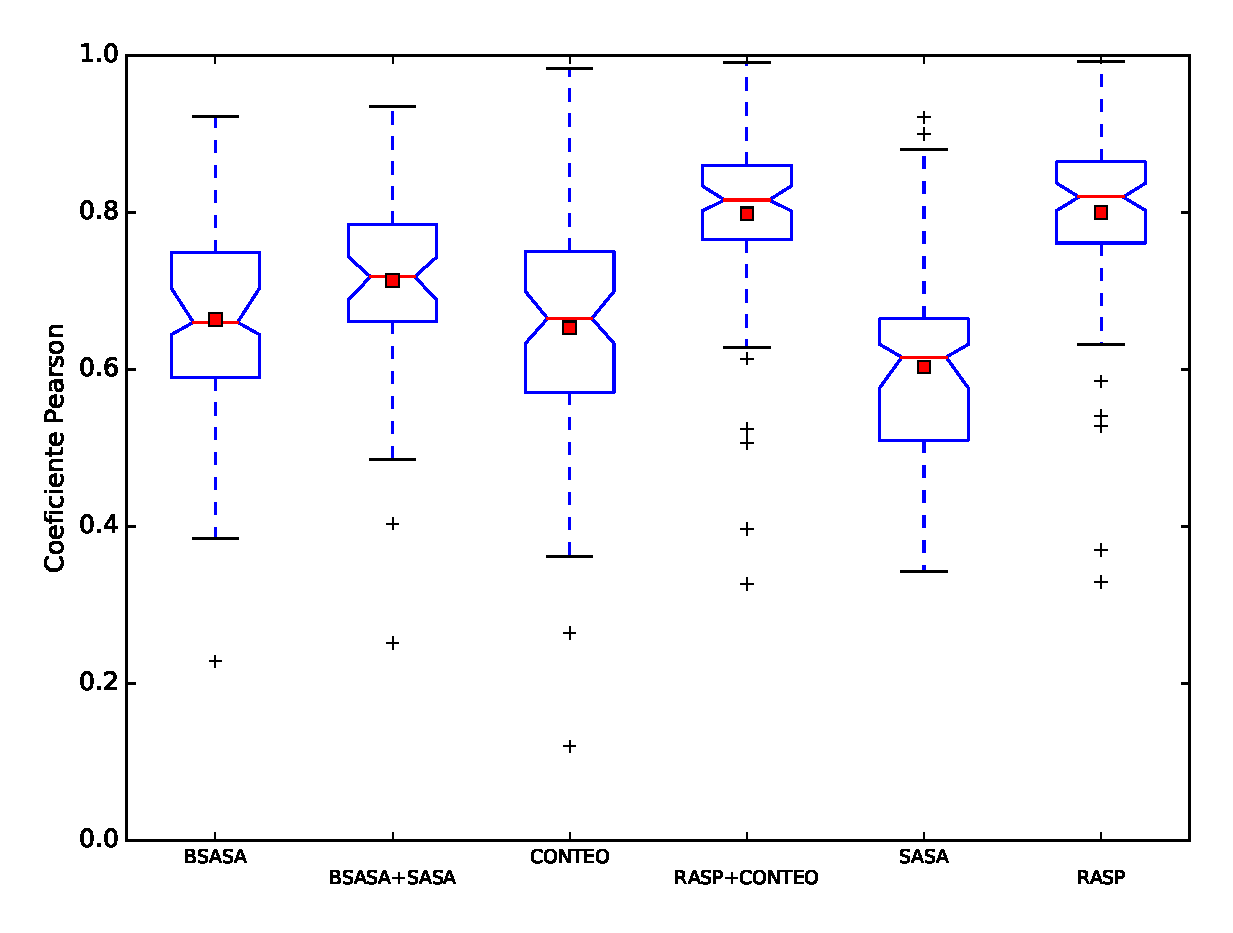
\includegraphics[width=\linewidth]{figures/resultados/rna/struct/boxplot_rmsd.eps}
    \caption{}
  \end{subfigure}
  \begin{subfigure}{.8\linewidth}
    \centering
    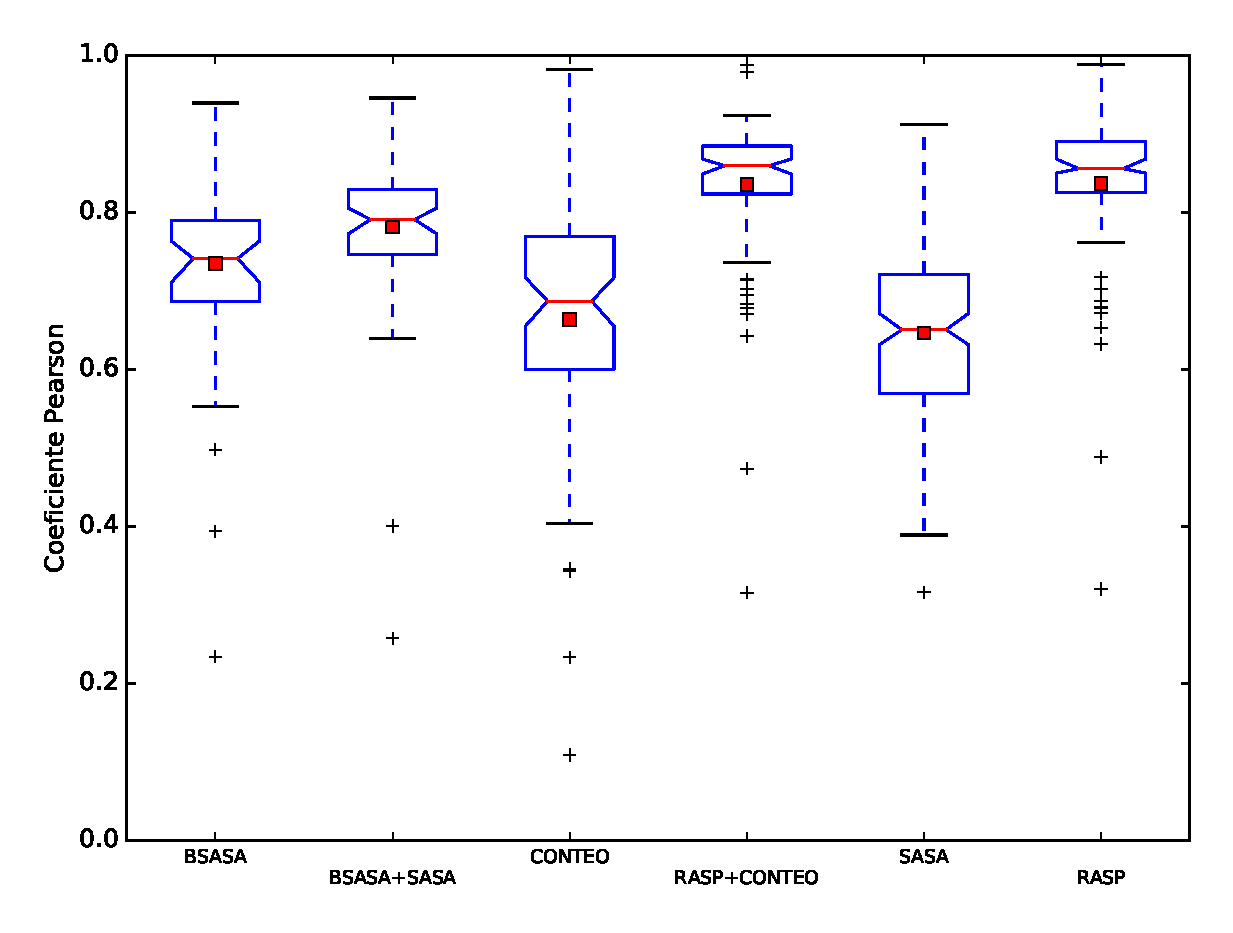
\includegraphics[width=\linewidth]{figures/resultados/rna/struct/boxplot_gdt.eps}
    \caption{}
  \end{subfigure}
 
\caption[Boxplots de las distribuciones de correlación de desviación estructural en RNA con un potencial.]{Boxplots de las distribuciones de correlación de desviación estructural en RNA con un potencial. En la figura (a) se tienen las correlaciones entre los valores de energía calculados por los potenciales evaluados y el RMSD, mientras que en (b) se tiene la correlación entre estos valores de energía y el GDT. La línea roja indica la mediana, el cuadrado rojo el promedio y la cintura el intervalo de confianza de la mediana. El N de cada boxplot es de 84.}
\label{fig:cap2011}
\end{figure}

\begin{table}[!htp]
\begin{tabular}{p{78pt} p{78pt} p{35pt} p{70pt} p{29pt} p{40pt} p{20pt}}
\hline \\
\textbf{RMSD}& RASP+CONTEO & BSASA    & BSASA+SASA &  RASP    & CONTEO   & SASA \\
RASP+CONTEO  & -           & -        & -          & -        & -        & -    \\
BSASA        & \textbf{$<$0.001}    & -        & -          & -        & -        & -    \\
BSASA+SASA   & \textbf{$<$0.001}    & \textbf{$<$0.001} & -          & -        & -        & -    \\
RASP         & \textbf{$<$0.001}    & \textbf{$<$0.001} & \textbf{$<$0.001}   & -        & -        & -    \\
CONTEO       & \textbf{$<$0.001}    & 0.4914   & $<$0.001   & \textbf{$<$0.001} & -        & -    \\
SASA         & \textbf{$<$0.001}    & \textbf{$<$0.001} & \textbf{$<$0.001}   & \textbf{$<$0.001} & \textbf{$<$0.001} & -    \\
\hline
\end{tabular}
\begin{tabular}{p{78pt} p{78pt} p{35pt} p{70pt} p{29pt} p{40pt} p{20pt}}
\hline \\
\textbf{GDT} & RASP+CONTEO & BSASA    & BSASA+SASA & RASP     & CONTEO   & SASA \\
RASP+CONTEO  & -           & -        & -          & -        & -        & -    \\
BSASA        & \textbf{$<$0.001}    & -        & -          & -        & -        & -    \\
BSASA+SASA   & \textbf{$<$0.001}    & \textbf{$<$0.001} & -          & -        & -        & -    \\
RASP         & 0.1828      & \textbf{$<$0.001} & \textbf{$<$0.001}   & -        & -        & -    \\
CONTEO       & \textbf{$<$0.001}    & \textbf{$<$0.001} & \textbf{$<$0.001}   & \textbf{$<$0.001} & -        & -    \\
SASA         & \textbf{$<$0.001}    & \textbf{$<$0.001} & \textbf{$<$0.001}   & \textbf{$<$0.001} & 0.0619   & -    \\
\hline
\end{tabular}
\caption[Comparación entre distribuciones de coeficientes de Pearson para correlaciones entre energía y desviación estructural en ARN.]{Comparación entre distribuciones de coeficientes de Pearson para correlaciones entre energía y desviación estructural en ARN para las medidas de RMSD y GDT. Los valorse en la tabla son los p-value de la prueba de Wilcoxon. Valores de p-value menores a 0.05 indican que la distribución es significativamente distinta.}
\label{table:cap2011res}
\end{table}

\subsubsection{Desempeño en encontrar el mejor modelo no canónico}
\par
En esta prueba se evaluó la capacidad de los nuevos potenciales en encontrar el mejor modelo de RNA con interacciones no canónicas, como fue descrito en la metodología.
En la figura~\ref{fig:farfar1} se tienen gráficos que indican en cuáles de los 32 casos posibles cada par de potenciales encuentra un peor o mejor modelo. Se puede observar que el potencial de superficie SASA supera al potencial CONTEO y que el potencial combinado BSASA+SASA supera al potencial utilizando la metodología antigua RASP+CONTEO.
\par
En la tabla~\ref{table:farfar} tenemos destacado las oportunidades en que un potencial logró encontrar el modelo con el mejor RMSD para cada estructura, cuyo valor está en la última columna.
El potencial BSASA+SASA logra 10 aciertos, contra solo 6 del potencial RASP+CONTEO.
Entre tanto el potencial RASP solo logra 8 aciertos contra los 7 de BSASA, y en los potenciales de superficie SASA logra 8 aciertos contra solo 4 de CONTEO.

\begin{figure}[hp] 
  \begin{subfigure}{.55\linewidth}
    \centering 
    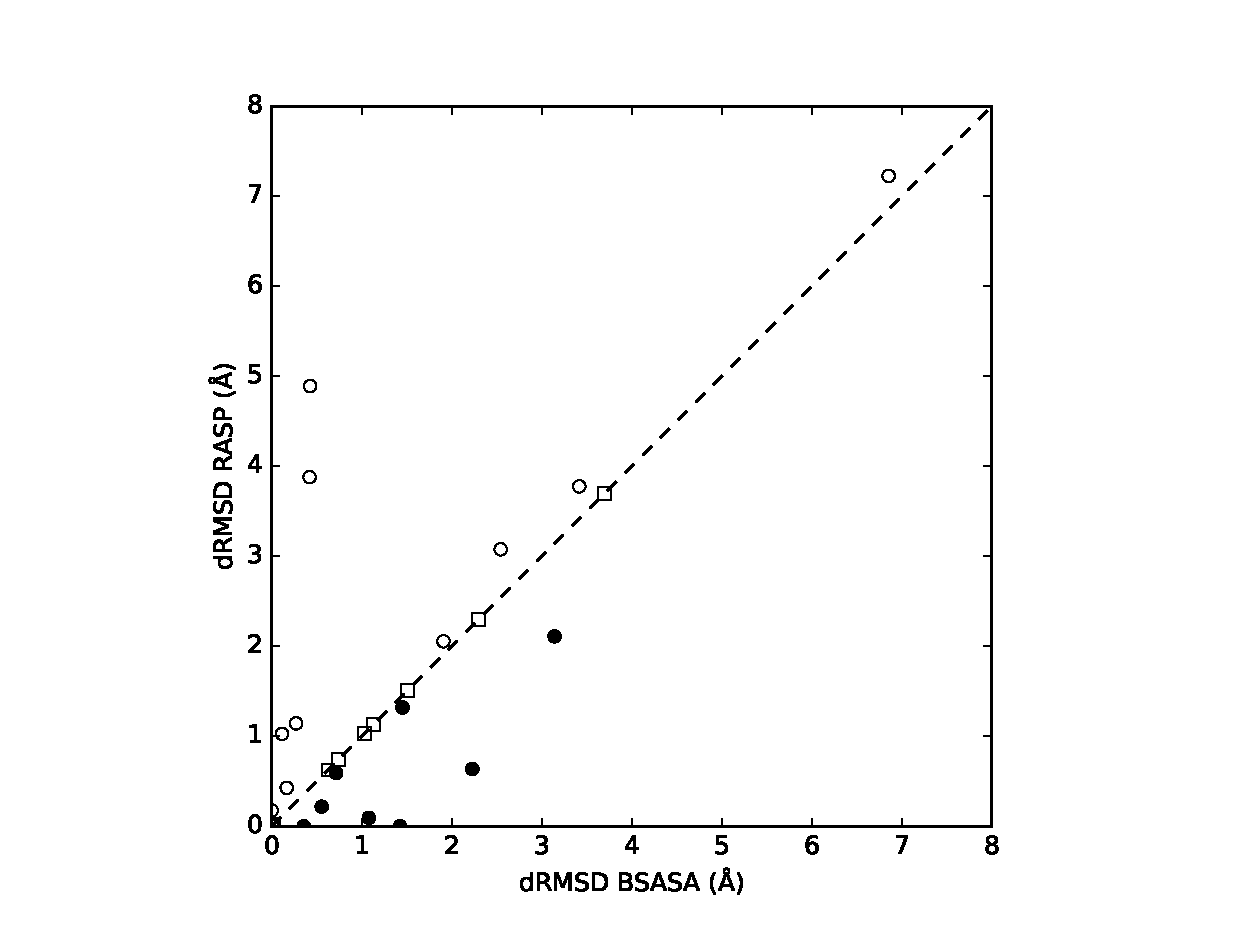
\includegraphics[width=\linewidth]{figures/resultados/rna/farfar/drmsd/BSASA_RASP_.eps}
    \caption{}
  \end{subfigure}%
~
  \begin{subfigure}{.55\linewidth}
    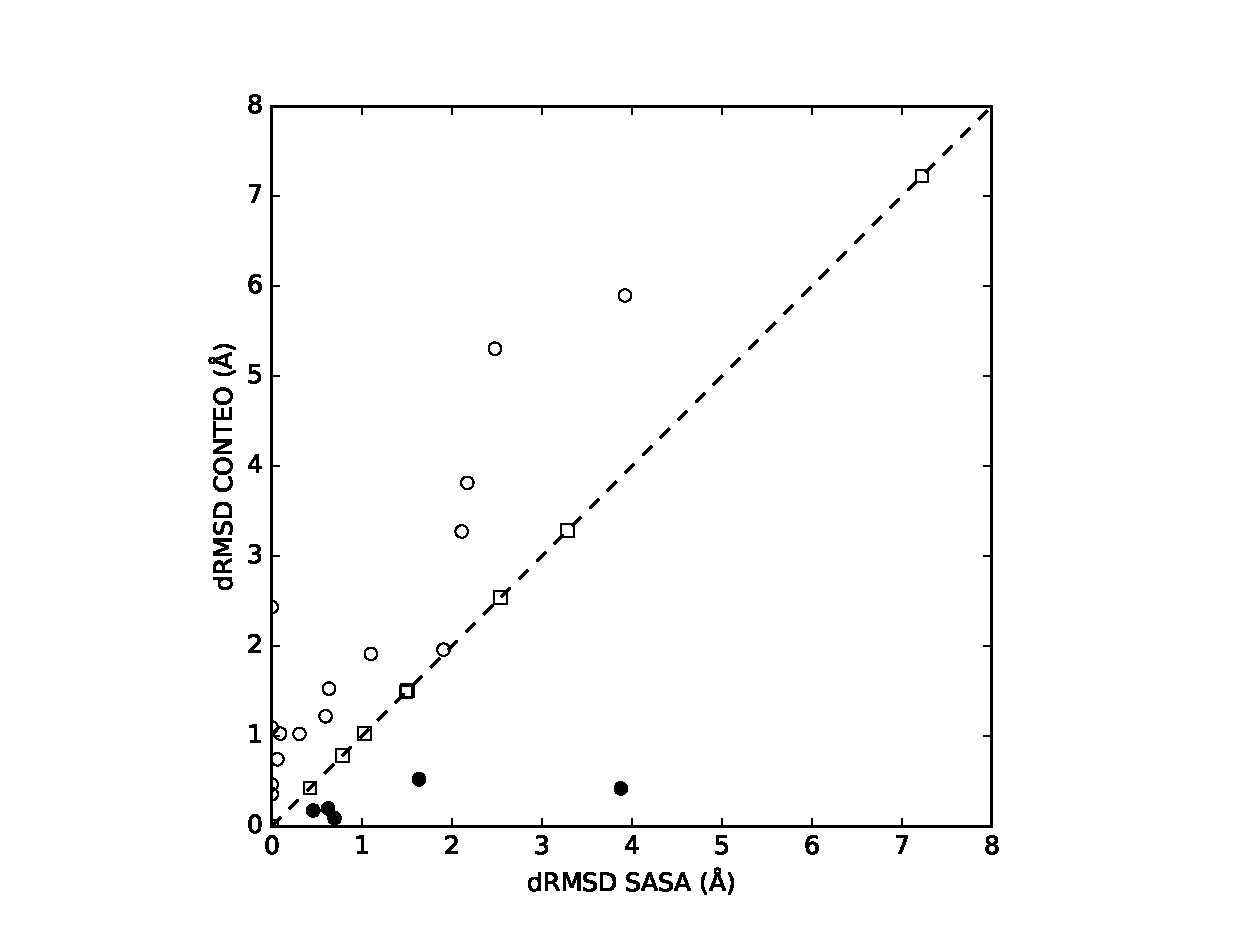
\includegraphics[width=\linewidth]{figures/resultados/rna/farfar/drmsd/SASA_CONTEO_.eps}
    \caption{}
  \end{subfigure}

  \begin{subfigure}{.55\linewidth}
    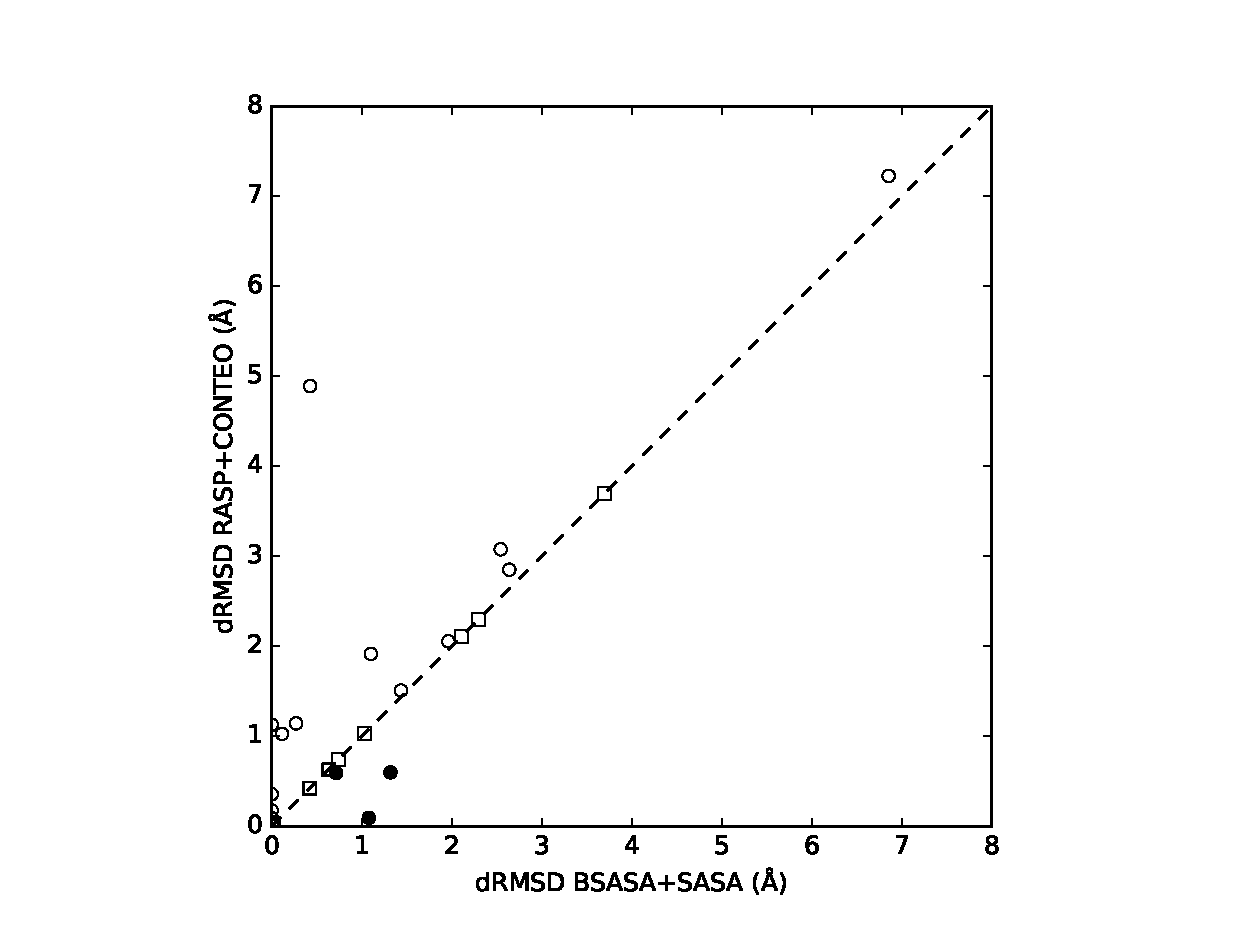
\includegraphics[width=\linewidth]{figures/resultados/rna/farfar/drmsd/BSASA+SASA_RASP+CONTEO_.eps}
    \caption{}
  \end{subfigure}

\caption[Comparación de las diferencias de RMSD entre el modelo de menor RMSD y el modelo de menor energía encontrado por el potencial.]{Comparación de las diferencias de RMSD entre el modelo de menor RMSD y el modelo de menor energía encontrado por el potencial. En cada gráfico los puntos negros corresponden a los casos donde el potencial en el eje Y seleccionó un modelo más preciso que el potencial en el eje X. Los puntos blancos indican lo contrario de lo anterior, y los cuadrados blancos indican que ambos potenciales encontraron el mismo resultado. En (a) se tiene la comparación entre los potenciales RASP y BSASA, en (b) entre los potenciales CONTEO y SASA, y en (c) entre los potenciales combinados RASP+CONTEO y BSASA+SASA.
Los gráficos utilizan los datos de la tabla~\ref{table:farfar}.}
\label{fig:farfar1}
\end{figure}

\begin{table}[!htp]
\begin{tabular}{p{48pt}|p{40pt} p{40pt} p{40pt} p{43pt} p{47pt} p{49pt} p{43pt}}
PDB ID& BSASA& RASP& SASA& CONTEO& BSASA+ SASA& RASP+ CONTEO& MEJOR RMSD \\
\hline \\
2gis-003 & 8.075 & 8.447& 8.447& 8.447& 8.075& 8.447& \textbf{1.22}\\
2oeu-002 & 9.863& 9.863& 8.193& 7.764& 9.863& 9.863& \textbf{7.565}\\
157d-001 & \textbf{1.19} & \textbf{1.19} &2.292& 3.106 &2.292 &3.106 & \textbf{1.19}\\
2r8s-003 & 2.475 & 2.352 & \textbf{1.759} & 2.859 & 2.475 & 2.352 & \textbf{1.759}\\
1kd5-001 & 4.044 & 2.451 & 2.451 & 3.344 & 2.451 & 2.451 & \textbf{1.814} \\
1xjr-003 & 4.142 & 3.109 & 3.11 & 4.275 & 3.109 & 3.109 & \textbf{0.999} \\
2eew-005 & 6.214 & 7.126 & 6.408 & 7.126 & 6.214 & 7.126 & \textbf{6.099} \\
1d4r-001 & \textbf{1.832} & \textbf{1.832} & 2.62 & 2.62 & \textbf{1.832} & \textbf{1.832} & \textbf{1.832} \\
2qwy-003 & 7.824 & 12.289 & 10.685 & 10.685 & 7.824 & 12.289 & \textbf{7.397} \\
1q9a-003 & \textbf{0.819} & \textbf{0.819} & \textbf{0.819} & \textbf{0.819} & \textbf{0.819} & \textbf{0.819} & \textbf{0.819} \\
2gdi-003 & \textbf{1.995} & \textbf{1.995} & \textbf{1.995} & \textbf{1.995} & \textbf{1.995} & \textbf{1.995} & \textbf{1.995} \\
1lnt-002 & 2.346 & 2.346 & \textbf{1.217} & 3.652 & \textbf{1.217} & 2.346 & \textbf{1.217} \\
2r8s-004 & 10.973 & 10.973 & 10.973 & 10.973 & 10.973 & 10.973 & \textbf{9.941} \\
1jj3-006 & 8.851 & 9.724 & 10.073 & 10.073 & 8.851 & 9.724 & \textbf{8.58} \\
2oiu-013 & 1.214 & \textbf{0.857} & \textbf{0.857} & 1.214 & \textbf{0.857} & 1.214 & \textbf{0.857} \\
3b31-099 & 3.547 & 3.808 & 3.808 & 3.808 & 3.808 & 3.808 & \textbf{3.38} \\
1kh6-001 & 11.485 & 11.351 & 10.63 & 11.254 & 11.351 & 10.63 & \textbf{10.031} \\
lopE-099 & 2.269 & 2.269 & 3.278 & 2.163 & 2.269 & 2.269 & \textbf{1.641} \\
1mhk-001 & 5.136 & 5.495 & 5.643 & 7.616 & 4.358 & 4.569 & \textbf{1.718} \\
255d-002 & \textbf{2.095} & \textbf{2.095} & \textbf{2.095} & 2.559 & \textbf{2.095} & \textbf{2.095} & \textbf{2.095} \\
1d4r-001 & 4.695 & \textbf{3.27} & \textbf{3.27} & \textbf{3.27} & \textbf{3.27} & \textbf{3.27} & \textbf{3.27} \\
uucg-005 & 1.148 & 1.148 & \textbf{1.122} & \textbf{1.122} & 1.148 & 1.148 & \textbf{1.122} \\
2qbz-099 & 4.507 & 3.523 & 3.523 & 4.458 & 4.507 & 3.523 & \textbf{3.428} \\
2r8s-004 & 3.312 & 6.77 & 6.77 & 3.312 & 3.312 & 3.312 & \textbf{2.891} \\
2oiu-002 & \textbf{2.24} & 2.416 & 2.702 & 2.416 & \textbf{2.24} & 2.416 & \textbf{2.24} \\
1q9a-001 & 5.16 & 5.16 & 3.634 & 5.277 & 5.16 & 5.16 & \textbf{1.46} \\
283d-001 & 1.743 & 1.743 & 1.062 & 1.743 & 1.743 & 1.743 & \textbf{0.998}\\
2oeu-003 & 11.187 & 11.721 & 11.187 & 11.187 & 11.187 & 11.721 & \textbf{8.643}\\
359d-001 & \textbf{7.659} & \textbf{7.659} & 10.139 & 12.966 & \textbf{7.659} & \textbf{7.659} & \textbf{7.659}\\
1u9s-001 & 3.293 & 3.44 & 3.293 & 3.347 & 3.347 & 3.44 & \textbf{1.384} \\
2eew-003 & 9.59 & 9.59 & 9.59 & 9.59 & 9.518 & 9.59 & \textbf{8.081} \\
1csl-002 & 4.415 & 4.078 & 4.557 & 3.949 & \textbf{3.859} & 3.949 & \textbf{3.859} \\
\hline
\end{tabular}
\caption[Tabla con los mejores RMSD encontrados para los 32 casos de estructuras no canónicas]{Tabla con los mejores RMSD encontrados por los potenciales para los 32 casos de estructuras no canónicas. El nuevo potencial BSASA+SASA logra encontrar 10 de los mejores casos, contra 8 de RASP y solo 6 de la combinación de RAS+CONTEO. En los potenciales de superficie, SASA supera a CONTEO con 8 modelos encontrados versus 4 para CONTEO.}
\label{table:farfar}
\end{table}

\cleardoublepage
\subsection{Pruebas en potenciales para ADN}
\subsubsection{Desempeño en la detección del modelo de menor RMSD}
\par
En esta prueba las capacidades de los potenciales en elegir los mejores modelos de ADN generados por el método de \cite{Ibarra2013} fueron comparadas utilizando las distribuciones de dRMSD, la diferencia entre el modelo encontrado por el potencial y el modelo original.
Esta prueba fue hecha con un set de modelos que fueron generados utilizando las restricciones espaciales calculadas por \cite{Ibarra2013}, y otro en el que estas fueron desactivadas.
\par
En la figura~\ref{fig:dna1} se observan los resultados para los dos conjuntos de modelos, mientras que en la tabla~\ref{table:dnacomp} podemos ver los resultados del test de Wilcoxon entre cada distribución de dRMSDs generada por los potenciales.
En el primer conjunto, figura~\ref{fig:dna1}a y tabla~\ref{table:dnacomp}a, podemos observar como aunque los potenciales BSASA y DD+CONTEO parecen tener mejor desempeño, de acuerdo al test estadistico todos estos potenciales son equivalentes.
Para el caso de la figura~\ref{fig:dna1}b y tabla~\ref{table:dnacomp}b, se pueden observar distribuciones muy parecidas a las anteriores, excepto para los potenciales SASA y CONTEO.
Pero de acuerdo al resultado de la comparación los únicos potenciales distintos son los pares DD/SASA y DD+CONTEO/SASA, en los cuáles los potenciales DD y DD+CONTEO tienen un mejor desempeño que SASA.
Las comparaciones entre los otros pares de potenciales no tuvieron diferencias significativas.

\begin{figure}[hp]
  \centering  
  \begin{subfigure}{.8\linewidth}
    \centering
    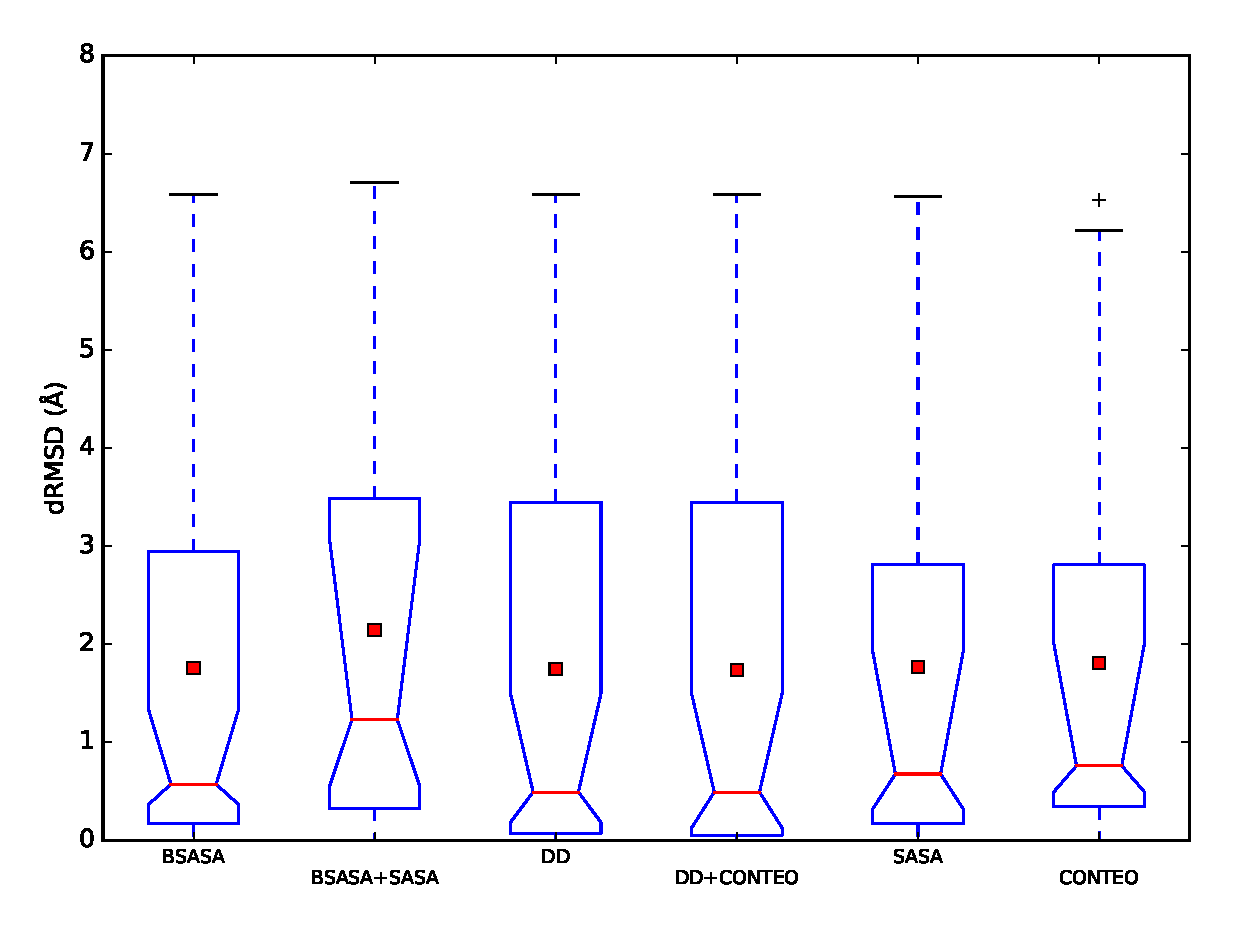
\includegraphics[width=\linewidth]{figures/resultados/dna/initial15.eps}
    \caption{}
  \end{subfigure}
  \begin{subfigure}{.8\linewidth}
    \centering
    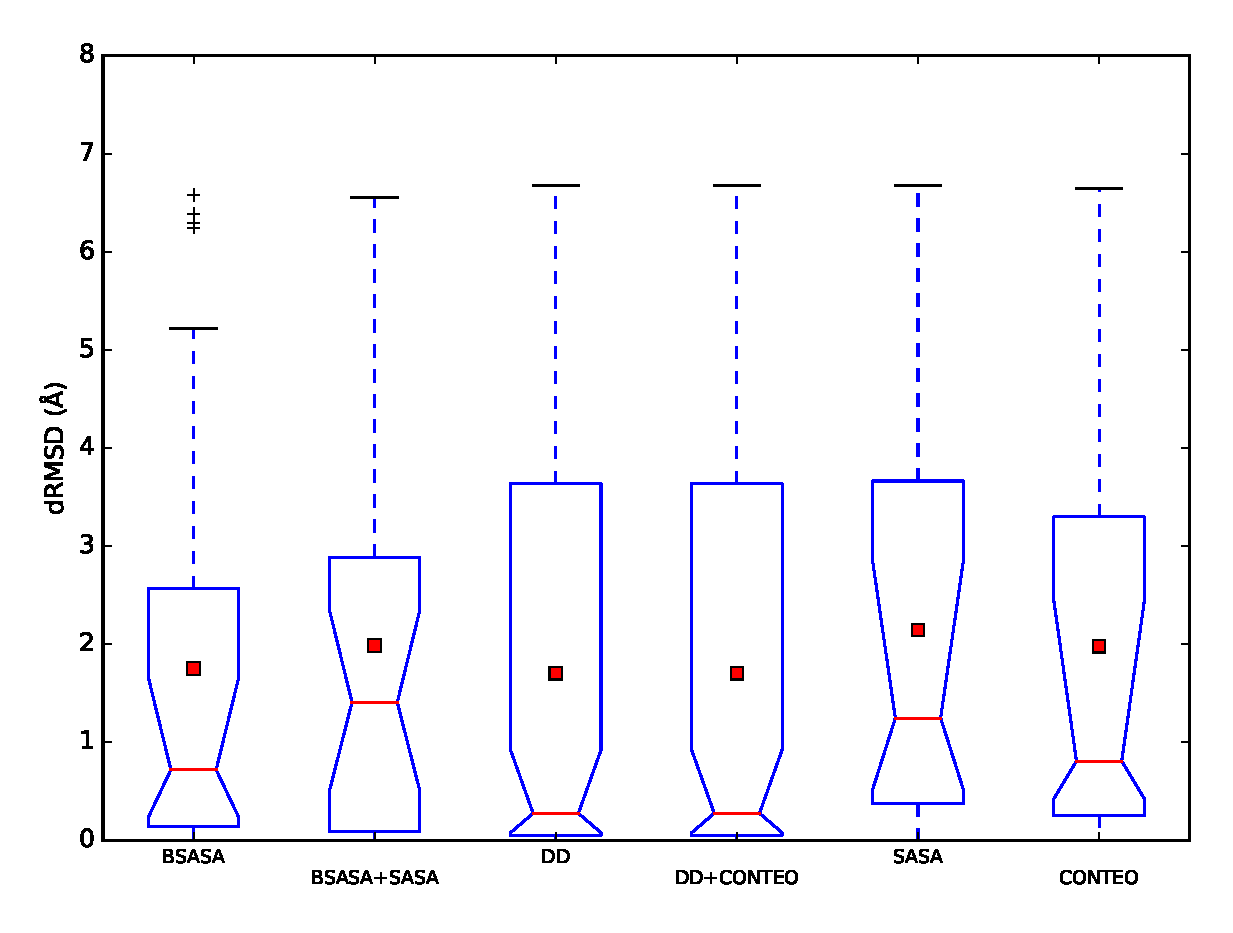
\includegraphics[width=\linewidth]{figures/resultados/dna/initial15_rsr_off.eps}
    \caption{}
  \end{subfigure}
 
\caption[Comparación de las distribuciones de dRMSD entre los modelos con menor RMSD y los modelos con menor energía calculado por cada potencial]{Comparación de las distribuciones de dRMSD entre los modelos con menor RMSD y los modelos con menor energía calculada por cada potencial. En la figura (a) tenemos los resultados calculados con los modelos con las restricciones activadas y en (b) con las restricciones activadas. La línea roja indica la mediana, el cuadrado rojo el promedio y la cintura el intervalo de confianza de la mediana. El N de cada boxplot es de 32.}
\label{fig:dna1}
\end{figure}

\begin{table}[!htp]
\begin{tabular}{p{78pt} p{78pt} p{40pt} p{70pt} p{25pt} p{39pt} p{20pt}}
\hline \\
\textbf{A}   & DD+CONTEO   & BSASA    & BSASA+SASA & DD       & CONTEO   & SASA \\
DD+CONTEO    & -           & -        & -          & -        & -        & -    \\
BSASA        & 0.793       & -        & -          & -        & -        & -    \\
BSASA+SASA   & 0.085       & 0.187    & -          & -        & -        & -    \\
DD           & 1.00        & 0.824    & 0.085      & -        & -        & -    \\
CONTEO       & 0.168       & 0.757    & 0.410      & 0.249    & -        & -    \\
SASA         & 0.418       & 0.976    & 0.368      & 0.516    & 0.338    & -    \\
\hline
\end{tabular}
\begin{tabular}{p{78pt} p{78pt} p{40pt} p{70pt} p{25pt} p{39pt} p{20pt}}
\hline \\
\textbf{B} & DD+CONTEO  & BSASA & BSASA+SASA & DD       & CONTEO   & SASA \\
DD+CONTEO    & -        & -     & -          & -        & -        & -    \\
BSASA        & 0.423    & -     & -          & -        & -        & -    \\
BSASA+SASA   & 0.134    & 0.285 & -          & -        & -        & -    \\
DD           & 1.0      & 0.424 & 0.134      & -        & -        & -    \\
CONTEO       & 0.081    & 0.285 & 0.771      & 0.081    & -        & -    \\
SASA         & \textbf{0.010}    & 0.059 & 0.285      & \textbf{0.010}    & 0.147    & -    \\
\hline
\end{tabular}
\caption[Tabla de comparaciones entre distribuciones de dRMSD entre pares de potenciales para los conjuntos de modelos de ADN con y sin restricciones.]{Tabla de comparaciones entre distribuciones de dRMSD entre pares de potenciales para los conjuntos de modelos de ADN con y sin restricciones. Los valores en la tabla son el p-value de la prueba de Wilcoxon. Valores menores a 0.05 indican que las distribuciones comparadas son significativamente distintas.}
\label{table:dnacomp}
\end{table}

